\chapter{Development Environment}\label{DevelEnv}

\section{Software Development Environment}

The software development environment that was chosen to create the
BALL compiler consists of Eclipse as the integretaged development evironment 
running on Ubuntu distribution of Linux OS. Ubuntu was chosen as the 
OS because it is open source and was readily available to all team members. 
Eclipse was chosen specifically because of its seamless integration with 
both Java and Subversion revision control system. The other tools selected
were chosen because they complemented Eclipse and Java natively.
Google Code was specially helpful in bringing everything
together since it made available to us features that were invaluable
at every stage of our compiler design. For the majority of the early
stages of our project, the record of our brainstorming sessions was
kept in a wiki stored on Google Code. This was a very helpful resource
that made it easy to trace the language and feature set
evolution. Likewise, without the ability to store our version
controlled code on Google Code, the development cycle would have been
extremely difficult to coordinate. In summary, the most important tools
used in the development of BALL were selected to leverage our team
members knowledge of Java.

\section{Software Development and Language Tools}
The Software Development tools are summarized below and illustrated in Figure \ref{toolsdiagram}

\begin{itemize}

\item Ubuntu Linux \item Java
\item Eclipse \item Google Code
\item Subversion \item JFlex
\item BYACC/J \item Apache Ant
\item LaTeX

\end{itemize}

\begin{figure}[htbp]
  \centering
  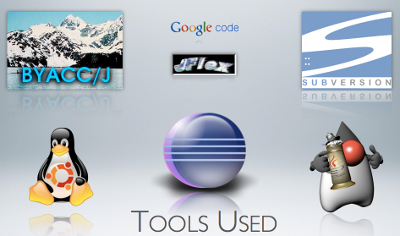
\includegraphics[scale=0.99]{softdevtools2.png}
  \caption{Tools Used}
  \label{toolsdiagram}
\end{figure}





\section{Implementation Languages and Tools}

Java was used to develop and build our BALL compiler to leverage the
considerable expertise that our team members possessed. It was also
specially helpful that Java is highly portable and enabled our BALL
compiler to work wherever Java runs. Only Java standard libraries were
used in the creation of our compiler, to simplify and further increase
the portability of BALL. Jflex \& BYACC/J the Java flavor versions of
Lex and Yacc were used to build our lexer and parser frontend. 
Apache Ant was used to write buildfiles that automated the compilation process 
of our Java package. A bash shell script tied it all together by calling our 
BALL compiler on BALL source files, compiling the generated intermediate Java
source code, and executing the Java bytecode. Finally, LaTex was used for the 
creation of the final report to achieve a professional look and design.
